\chapter{Arquitetura}

Este capítulo apresenta uma arquitetura de referência para cloud computing na primeira seção. Na seção final apresenta boas práticas e métodos para arquitetar uma aplicação que deve ser colocada em um ambiente de nuvem.

\section{Arquitetura de referência}

O objetivo da arquitetura de referência apresentada a seguir é de providenciar uma taxonomia simples e sem ambiguidade para os três modelos de serviço:

\begin{itemize}
  \item
    Software as a Service (SaaS)
  \item
    Platform as a Service (PaaS)
  \item
    Infrastructure as a Service (IaaS)
\end{itemize}

Tal arquitetura deve disponibilizar uma visão unificada das cinco características essenciais da NIST:

\begin{itemize}
  \item Serviço sobre demanda
  \item Amplo acesso à rede
  \item Agrupamento de recursos
  \item Elasticidade rápida (escalabilidade)
  \item Serviço mensurável
\end{itemize}

Após pesquisar informações disponibilizadas por provedores, instituições de pesquisa e de consultoria na área achamos interessante a seguinte arquitetura de referência:

\begin{figure}[h!]
  \centering
  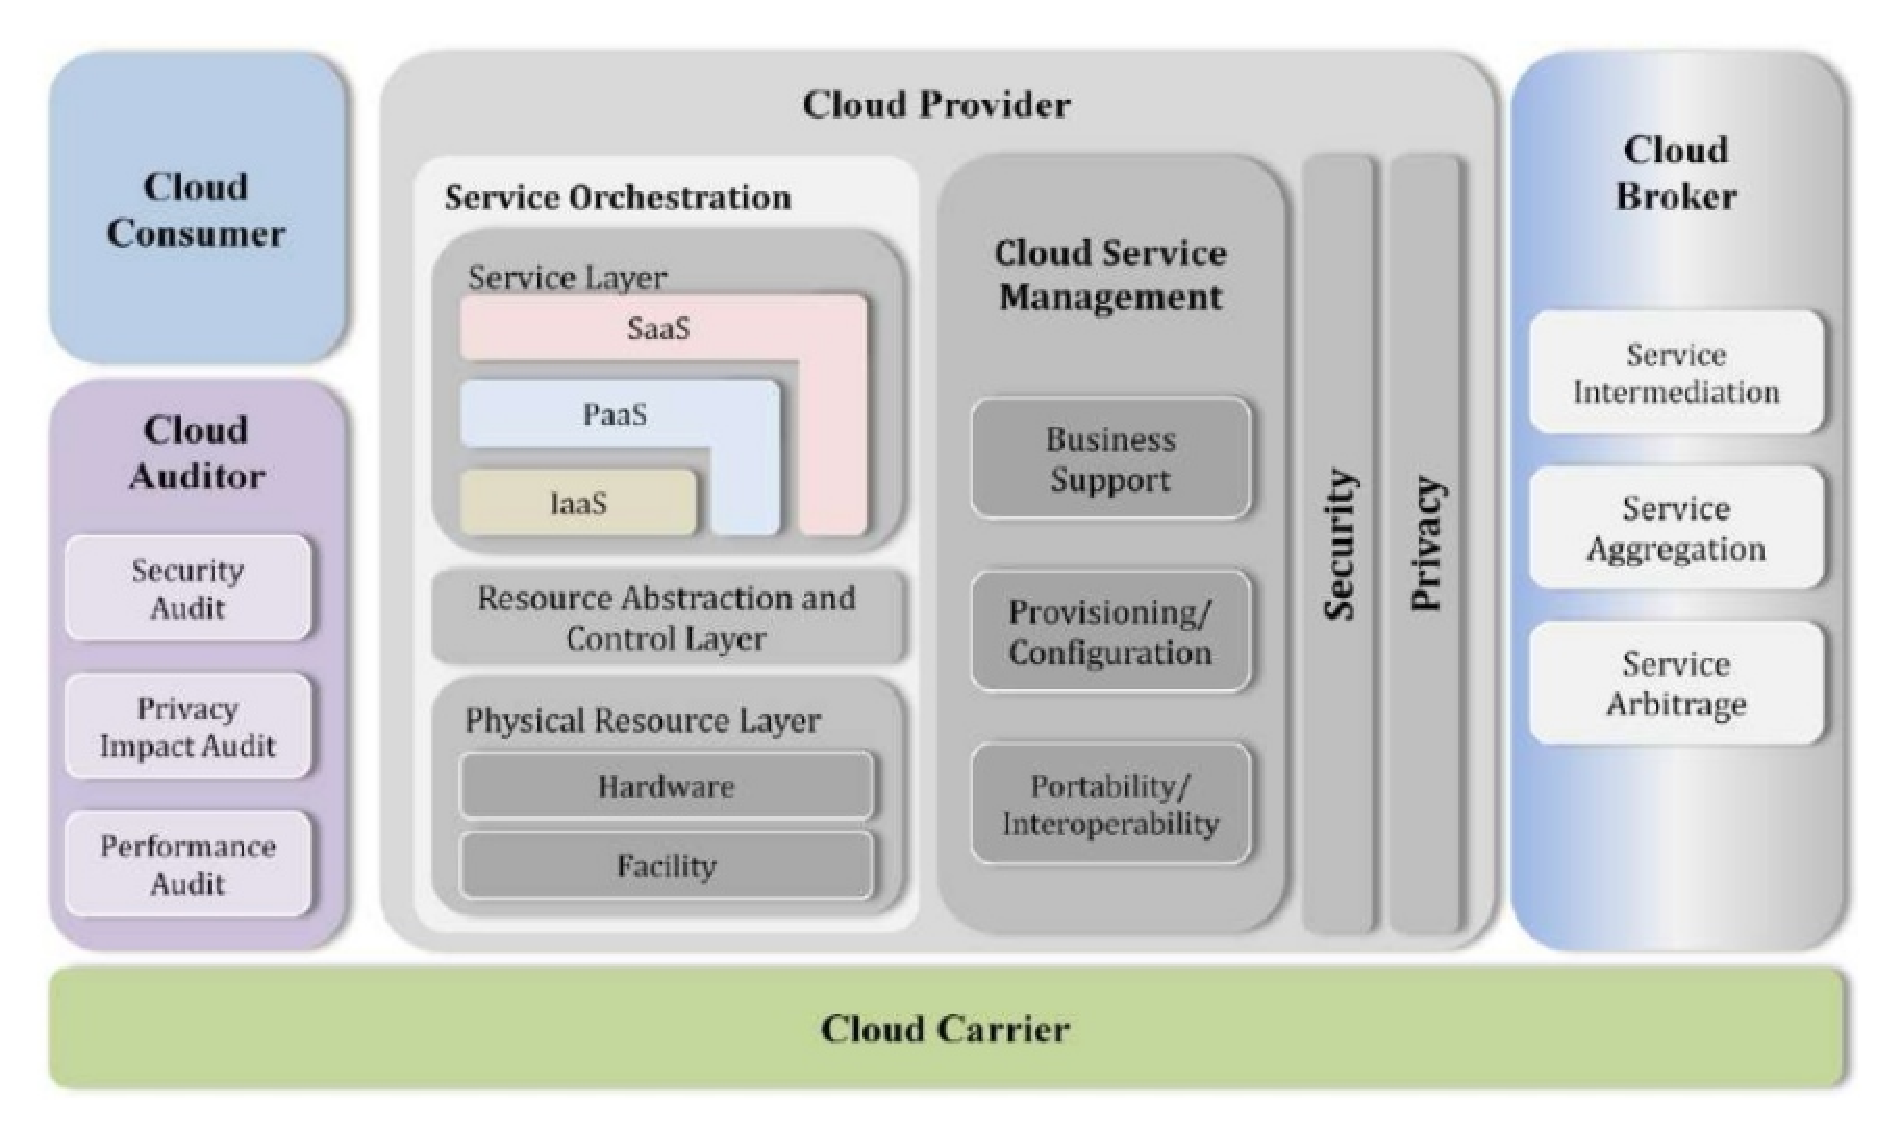
\includegraphics[scale=0.5]{imagens/cloudarch.eps}
  \caption{Arquitetura de referência para Cloud Computing}
\end{figure}

\subsection{Cloud Consumer}

Representa classes de consumidores para cada modelo possível de serviço. 

No caso de SaaS são diversos departamentos operacionais de uma empresa, consumindo serviços de ERP, CRM, vendas, finanças, RH, redes sociais, webmail etc. 

No caso de PaaS são os setores de análise de dados e desenvolvimento, que consomem serviços de BI, banco de dados, \textit{deployment} de aplicações, integração de sistemas e desenvolvimento e testes.

Por fim, os consumidores de IaaS são os setores da empresa responsável pela infraestrutura e IT, que consomem serviços de backup e recuperação, gerenciamento de serviços, armazenamento, hospedagem de plataformas etc.

\subsection{Cloud Auditor}

Cloud Auditor é o componente responsável por relatar e registrar as ações relativas a segurança, privacidade e performance da nuvem, tanto para fins de transparência para os consumidores quanto de regulamentação governamental para rastrear atividades suspeitas e irregulares. Pode ser tanto um órgão governamental ou uma entidade fiscalizadora global na Internet.

\subsection{Cloud Provider}

Cloud Provider é o provedor de nuvem como a \textit{Amazon Web Services}, \textit{Microsoft Azure}, \textit{Netflix}, \textit{Youtube}, dentre outros. Dependendo das categorias de modelo de serviço em que o provedor se encaixa, ele poderá ter camadas de serviço de SaaS, PaaS ou IaaS. 

As principais atividades do Cloud Provider são a implantação de serviços, a orquestração de serviços, o gerenciamento de serviços, a segurança e por fim, a privacidade. Deve gerenciar e abstrair toda lógica de controle e a camada física de recursos de hardware, bem como as instalações e locais físicos.

\subsection{Cloud Broker}

O Cloud Broker é responsável por uma espécie de serviço de corretagem. Este ator no ecossistema de nuvem é responsável por oferecer serviços de proteção jurídica durante a negociação de contratos com provedores de nuvem. 

Oferece também serviços de diminuição de custos com o provedor, agregando diversos serviços a fim de obter o melhor custo-benefício.

Por fim, pode oferecer serviços diferenciados, como um serviço adicional de segurança, para proteger o consumidor de vazamento de dados na nuvem.


\subsection{Cloud Carrier}

O Cloud Carrier são todas entidades responsáveis por disponibilizar a conexão e transporte de serviços na nuvem entre consumidores e provedores (Companhias de redes, telecomunicações, dispositivos de acesso e IoT).
